\documentclass{article}

% -------------------------------------------------
% Packages
% -------------------------------------------------

\usepackage{xcolor}
\usepackage{amsmath}
\usepackage{amssymb}
\usepackage{amsthm}
\usepackage{graphicx}
\usepackage{subcaption}
\usepackage{matlab-prettifier}
\usepackage{listings}
\usepackage{blindtext}
\usepackage{geometry}
\usepackage{float}
\usepackage{dirtytalk}
\usepackage{enumitem}
\usepackage{derivative}
\usepackage{biblatex}
\usepackage{svg}
\usepackage{hyperref}

% -------------------------------------------------
% Colors
% -------------------------------------------------

\definecolor{darkgreen}{rgb}{0.0, 0.5, 0.0}

% -------------------------------------------------
% Hyperlinks
% -------------------------------------------------

\hypersetup{
    colorlinks=true,
    linkcolor=blue,
    citecolor=blue,
    urlcolor=blue
}

% -------------------------------------------------
% Theorem environments
% -------------------------------------------------

% Numbered
\newtheorem{theorem}{Theorem}[section]
\newtheorem{lemma}[theorem]{Lemma}
\newtheorem{proposition}[theorem]{Proposition}

% Unnumbered
\newtheorem*{theorem*}{Theorem}
\newtheorem*{lemma*}{Lemma}
\newtheorem*{proposition*}{Proposition}

\theoremstyle{definition}
\newtheorem{definition}[theorem]{Definition}
\newtheorem{example}[theorem]{Example}

\theoremstyle{remark}
\newtheorem{remark}[theorem]{Remark}

% -------------------------------------------------
% Equation numbering
% -------------------------------------------------

% Reset equation numbering at each subsection
\makeatletter
\@addtoreset{equation}{subsection}
\makeatother

% If you want equations to be numbered by subsection,
% uncomment the following line:
% \renewcommand{\theequation}{\thesubsection.\arabic{equation}}

% -------------------------------------------------
% Python / MATLAB code formatting
% -------------------------------------------------

\lstset{
    language=Python,
    basicstyle=\ttfamily\small,
    keywordstyle=\color{blue},
    stringstyle=\color{darkgreen},
    commentstyle=\color{gray},
    showstringspaces=false,
    frame=single,
    numbers=left,
    numberstyle=\tiny\color{gray},
    breaklines=true
}

% -------------------------------------------------
% Page geometry
% -------------------------------------------------

\geometry{
    a4paper,
    total={160mm,250mm},
    left=25mm,
    top=30mm,
    footskip=10mm
}

% -------------------------------------------------
% Document settings
% -------------------------------------------------

\setlength{\parindent}{0pt}

% -------------------------------------------------
% Title
% -------------------------------------------------

\title{Statistical Models\\Assignment 1}
\author{Thomas Sejer Canham}
\date{\today}

% =================================================
% Document
% =================================================

\begin{document}

\maketitle

\section*{Introduction}

This assignment concerns maximum likelihood and asymptotic variance, and is motivated
by a real-world problem involving \textit{Salmonella enterica} in eggs.

Eggs are thought to be infected with a bacterium \textit{Salmonella enterica} so that
the number of organisms, $Y$, in each egg has a Poisson distribution with mean $\mu$.
The value of $Y$ cannot be observed directly, but after a period it becomes certain
whether the egg is infected ($Y>0$) or not ($Y=0$). Out of $m$ such eggs, $r$ are found
to be infected.


\subsection*{Question (a)} We wish to show that the maximum likelihood estimator $\hat{\mu}$ of $\mu$ is
\[
    \hat{\mu}
    =
    \log\left(\frac{m}{m-r}\right).
\]
We consider the event $P(Y_i > 0)$, where $Y_i \sim Poisson(\mu)$ is the number of organisms in the $i$-th egg, and we may state the number of infected eggs as.
\[
    R = \sum_{i=1}^{m} \mathbf{1}(Y_i>0).
\]
The probability $P(Y_i>0) = 1 - P(Y_i \leq 0)$ can be calculated from the CDF of the Poisson distribution
\[
 1 - e^{-\mu}\sum_{j=0}^0 \frac{ \mu^j}{j!} = 1 - e^{-\mu}.
\]
So $R$ is the sum of $m$ independent Bernoulli random variables with success probability $p(\mu) = 1 - e^{-\mu}$. Thus $R$ has a binomial distribution with parameters $m$ and $p$. The MLE for a binomial distribution is the fractions of succesful trials to the total number of trials. Note that $p(\mu)$ is a strictly monotone function of $\mu$, as such we can find $\hat \mu = f^{-1}(\hat p)$ and the inverse is guaranted to exist.


\begin{equation}
    \hat p = \dfrac{r}{m} \iff 1 - e^{-\hat \mu} = \dfrac{r}{m} \iff e^{-\hat \mu} = 1-\dfrac{r}{m} \iff e^{-\hat \mu} = \dfrac{m-r}{m} \iff \hat \mu = \log(\dfrac{m}{m-r})
\end{equation}
$\square$
\subsection*{Question (b)}
Since $R$ is a sample with just one realization the likelihood function is given by the probability mass function of the binomial distribution, let $c = \binom{m}{r}$, then the likelihood function is
\[
    L(p) = P(R=r) =c p^r(1-p)^{m-r}.
\]
with log-likelihood function
\[
    \ell(p) = \log L(p) = \log c + r\log p + (m-r)\log(1-p).
\]
If we substitute $p = 1 - e^{-\mu}$ we get
\[
    \ell(\mu) = \log c + r\log(1 - e^{-\mu}) + (m-r)\log(e^{-\mu}) = \log c + r\log(1 - e^{-\mu}) - (m-r)\mu.
\]
The score function is given by the derivative of the log-likelihood function with respect to $\mu$,
\[
    S(\mu) = \frac{d\ell}{d\mu} = \frac{re^{-\mu}}{1 - e^{-\mu}} - (m-r).
\]
We then find the second derivative of the log-likelihood function with respect to $\mu$,
\[
    \frac{d^2\ell}{d\mu^2} = \frac{dS(\mu)}{d\mu} = \frac{-re^{-\mu}(1 - e^{-\mu}) -re^{-\mu} e^{-\mu} }{(1 - e^{-\mu})^2} = \frac{-re^{-\mu}}{(1 - e^{-\mu})^2}.
\]
The Fisher information is given by the negative expected value of the second derivative of the log-likelihood function with respect to $\mu$,
\[
    I(\mu) = E\left[-\frac{d^2\ell(\mu)}{d\mu^2}\right] = E[\frac{Re^{-\mu}}{(1 - e^{-\mu})^2}] = \frac{e^{-\mu}}{(1 - e^{-\mu})^2}E[R] = \frac{e^{-\mu}}{(1 - e^{-\mu})^2}mp
\]
Since $p = 1 - e^{-\mu}$ we have
\[
    I(\mu) = \frac{e^{-\mu}}{(1 - e^{-\mu})^2}m(1 - e^{-\mu}) = \frac{me^{-\mu}}{1 - e^{-\mu}}.
\]
Since our entire sample consists of just one realization of $R$, the asymptotic variance of $\hat{\mu}$ is given by the inverse of the Fisher information,
\[
    \text{Var}(\hat{\mu}) = I(\mu)^{-1} = \frac{1 - e^{-\mu}}{me^{-\mu}}   = \frac{e^{\mu} - 1}{m} 
\]
$\square$


\subsection*{Question (c)}

We run simulations to estimate the mean and variance of $\hat{\mu}$, and to plot the empirical CDF of $\hat{\mu}$. We use $Nsim = 10000$ simulations, with $m = 20$ eggs and $\mu = 2$. I find the estimated mean and variance:
\begin{equation}
    \hat{\mu} = 2.08, \quad \text{Var}(\hat{\mu}) \approx 0.299
\end{equation}
Note that since we have a large number of simulations, we will sometimes hit a sample where all eggs are infected, i.e. $r = m$. In this case we have a division by zero error when calculating $\hat{\mu}$, and we simply skip that sample.


\begin{figure}[H]
    \centering
    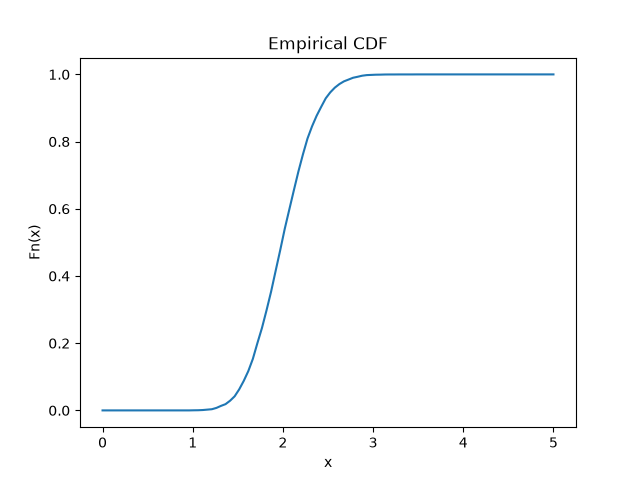
\includegraphics[width=0.7\textwidth]{CDF.png}
    \caption{Empirical CDF of $\hat{\mu}$.}
    \label{fig:CDF}
\end{figure}
The code for the simulations is shown below.
\begin{lstlisting}
import numpy as np
import matplotlib.pyplot as plt
np.random.seed(1)
Nsim = 10000
m = 20
mu = 2
xrange = np.linspace(0,5,100)

means = []

for i in range(Nsim):
    # Unobservable Poission
    y = np.random.poisson(mu, m)
    # How many of the eggs have bacteria?
    r = sum([1 if yi > 0 else 0 for yi in y])
    # Division by zero error!
    try:
        mu_hat = np.log(m / (m-r))
    except ZeroDivisionError:
        continue
    means.append(mu_hat)


Femp = lambda means: [np.sum(means < x) / len(means) for x in xrange]
print("Estimated mean: ", np.mean(means))
print("Estimated variance: ", np.var(means))
theoretical_var = (np.exp(mu) - 1) / m
print("Theoretical variance: ", theoretical_var)

plt.plot(xrange,Femp(means))
plt.xlabel("x")
plt.ylabel("Fn(x)")
plt.title("Empirical CDF")
plt.savefig("CDF2.png")
plt.close()

\end{lstlisting}
 The empirical CDF of $\hat{\mu}$ is shown in Figure \ref{fig:CDF}, and has a striking resemblance to the theoretical CDF for a normal distribution.

\subsection*{Question (d)}
We now redo the simulations with $m = 200$ eggs, we get the CDF in Figure \ref{fig:CDF2}. The estimated mean and variance are
\begin{equation}
    \hat{\mu} = 2.016, \quad \text{Var}(\hat{\mu}) \approx 0.034
\end{equation}
The theoretical variance is given by
\begin{equation}
    \text{Var}(\hat{\mu}) = \frac{e^{\mu} - 1}{m} = \frac{e^{2} - 1}{200} \approx 0.0319
\end{equation}
We see that the CDF steepens around the true value of $\mu = 2$, and the estimated variance is closer to the theoretical variance. This is consistent with the asymptotic normality of $\hat{\mu}$, as we have increased the sample size $m$.

\begin{figure}[H]
    \centering
    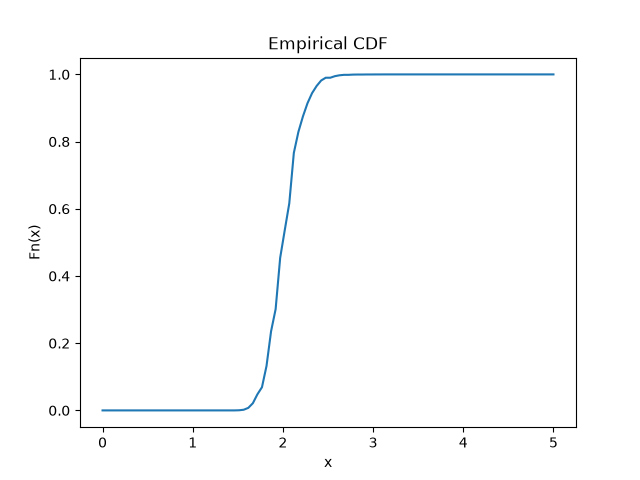
\includegraphics[width=0.7\textwidth]{CDF2.png}
    \caption{Empirical CDF of $\hat{\mu}$ with $m = 200$.}
    \label{fig:CDF2}
\end{figure}

\subsection*{Question (e)}
We now address division by zero errors. Due to the finite sample size and non-zero probability of having all eggs infected, we will sometimes hit a sample where $r = m$. According to our model this is a Binomaial experiment with only successes, thus the probabiltiity of this event is given by
\[
    P(R = m) = p^m = (1 - e^{-\mu})^m
\]
Since $e^x > 0$ for all $x \in \mathbb{R}$, we have that $(1 - e^{-\mu}) < 1$ for all $\mu > 0$. Thus, if we increase the sample size $m$, the probability of division by zero errors decreases exponentially, so
\begin{equation}
    P(R = m) = (1 - e^{-\mu})^m \to 0 \quad \text{as} \quad m \to \infty.
\end{equation}
Therefore, the probability of division by zero errors approaches zero as the sample size $m$ increases - which is consistent with the asymptotic normality of $\hat{\mu}$. However, it highligts issues with finite sample approximations. We illustrate this in the QQ-plots in Figure \ref{fig:QQ}.We see that the normal approximation of $\hat{\mu}$ improves as $m$ increases. The code for the QQ-plots is shown below.
\begin{lstlisting}
from scipy.stats import probplot
plt.figure(figsize=(12, 10))

for j, m in enumerate([20, 50, 100, 500]):
    mu_hats = []
    for i in range(Nsim):
        y = np.random.poisson(mu, m)
        r = sum([1 if yi > 0 else 0 for yi in y])
        try:
            mu_hat = np.log(m / (m - r))
        except ZeroDivisionError:
            continue
        mu_hats.append(mu_hat)

    plt.subplot(2, 2, j + 1)
    probplot(mu_hats, dist="norm", plot=plt)
    plt.title(f"Normal Q-Q plot, m = {m}")

plt.tight_layout()
plt.savefig("QQ.png")
plt.show()
\end{lstlisting}


\begin{figure}[H]
    \centering
    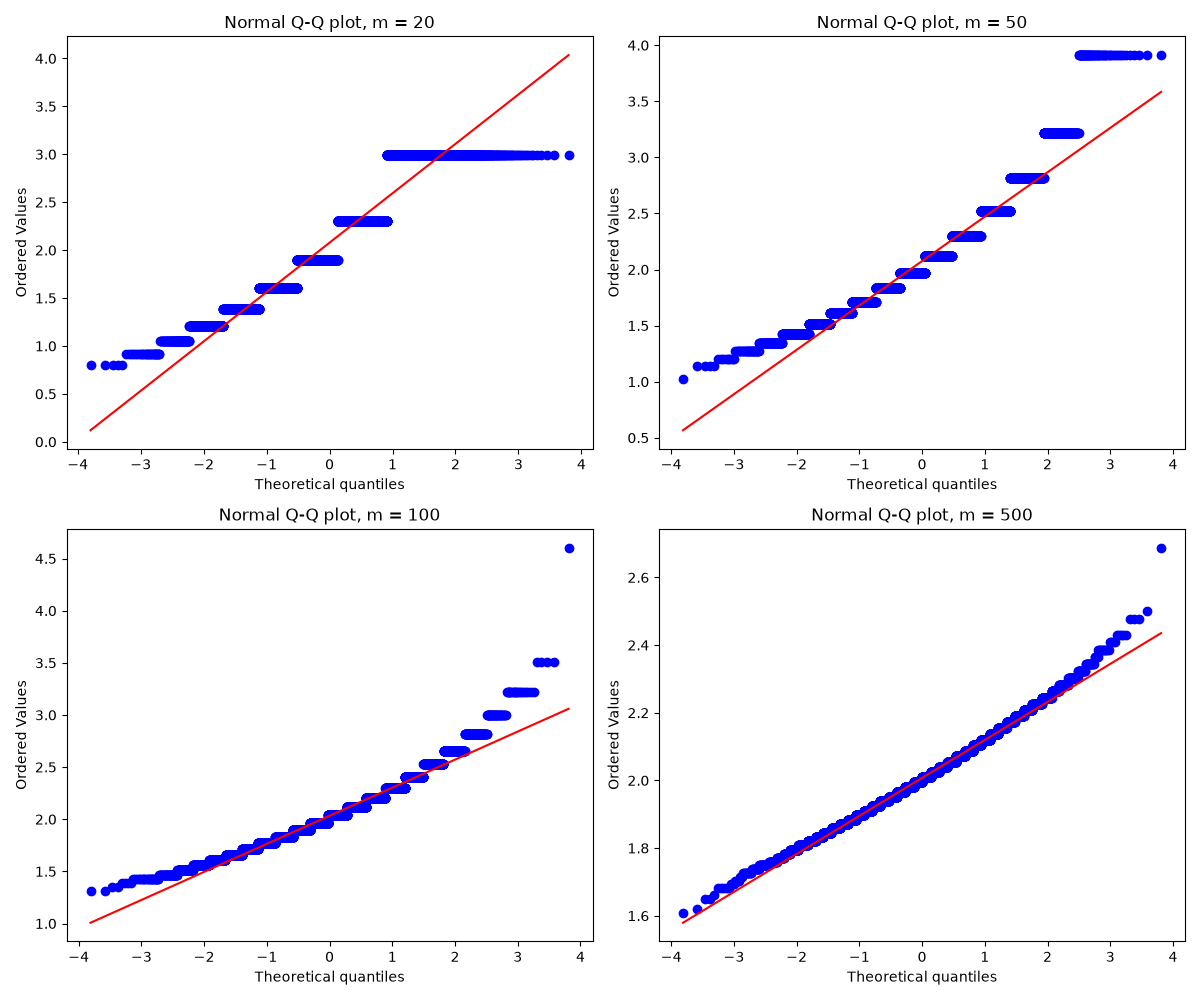
\includegraphics[width=0.9\textwidth]{QQ.png}
    \caption{QQ-plots at $m= 20,50, 100, 500$}
    \label{fig:QQ}
\end{figure}



\end{document}
